% Nota: Asegúrate de incluir \usepackage{tikz} en el preámbulo de tu documento.
\textbf{02/10/2026}
\section{Espacios simplemente conexos, deformación de aplicaciones y grupo fundamental de $S^n$}

\begin{observacion}{}{}
Recordamos que si $X \simeq Y$, entonces $\pi_1(X) \cong \pi_1(Y)$ suponiendo que $X$ e $Y$ son arco-conexos.
Como consecuencia, si $X$ es contractible (es decir, $X \simeq \{p\}$), entonces se tiene que $\pi_1(X) = 1$.
\end{observacion}

\begin{definicion}{Espacio simplemente conexo}{def_simp_conexo}
Sea $X$ un espacio topológico. Diremos que $X$ es simplemente conexo cuando es arco-conexo y $\pi_1(X) = 1$.
\end{definicion}

\begin{proposicion}{}{prop_arco_conexo}
Sea $X$ un espacio arco-conexo. Entonces:

$$\pi_1(X) = 1 \iff \forall x_0, x_1 \in X, \forall \alpha, \beta \in C_{x_0, x_1}(X) : \alpha \simeq_{\{0,1\}} \beta$$
\end{proposicion}

\begin{proof}
$\Rightarrow)$ Sean $x_0, x_1 \in X$ y sean $\alpha, \beta \in C_{x_0, x_1}(X)$. 

\begin{figure}[htbp]
\centering
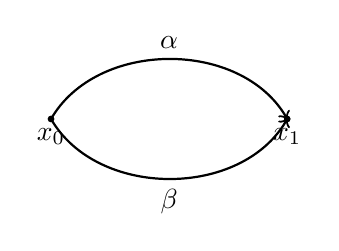
\begin{tikzpicture}
  \coordinate (X0) at (0,0);
  \coordinate (X1) at (3,0);
  \filldraw (X0) circle (1pt) node[below] {$x_0$};
  \filldraw (X1) circle (1pt) node[below] {$x_1$};
  \draw[thick, ->] (X0) to[out=60,in=120] node[above] {$\alpha$} (X1);
  \draw[thick, ->] (X0) to[out=-60,in=-120] node[below] {$\beta$} (X1);
\end{tikzpicture}
\caption{Lazos homotópicos $\alpha$ y $\beta$ entre $x_0$ y $x_1$.}
\end{figure}

Como $X$ es arco-conexo y $\pi_1(X) \cong \pi_1(X, x_0) = 1 = [c_{x_0}]$, consideramos el lazo $f := \alpha * \overline{\beta} \in C_{x_0, x_0}(X)$.
Dado que $\pi_1(X) = 1$, se cumple que $[\alpha * \overline{\beta}] = 1$. Esto implica que $[\alpha] \cdot [\beta^{-1}] = 1$, y por tanto $[\alpha] = [c_{x_0} * \beta] = [\beta]$ y por consiguiente $\alpha \simeq_{\{0,1\}} \beta$.

$\Leftarrow)$ Trivial tomando $x_0 = x_1$.
\end{proof}

\begin{proposicion}{}{prop_reparametrizacion}
Sea $g: I \longrightarrow I$ una aplicación continua tal que $g(0)=0$ y $g(1)=1$. Sea $\alpha: I \longrightarrow X$ una aplicación continua, siendo $X$ un espacio topológico cualquiera. Entonces se cumple que $\alpha \simeq_{\{0,1\}} \alpha \circ g$.
\end{proposicion}
\begin{figure}[htbp]
\centering
\begin{tikzpicture}[scale=1.5]
  \draw[->] (-0.2,0) -- (1.5,0);
  \draw[->] (0,-0.2) -- (0,1.5);
  \draw (1,0.05) -- (1,-0.05) node[below] {$1$};
  \draw (0.05,1) -- (-0.05,1) node[left] {$1$};
  \draw[blue, thick] (0,0) .. controls (0.2,0.8) and (0.6,0.3) .. (1,1);
\end{tikzpicture}
\caption{Gráfica de la reparametrización continua $g: I \longrightarrow I$.}
\end{figure}
\begin{proof}
Sea $F: I \times I \longrightarrow X$ la aplicación continua definida por $F(s,t) = \alpha((1-t)s + t g(s))$. Comprobamos sus valores:
\begin{itemize}
\item $F_0(s) = F(s,0) = \alpha((1-0)s + 0 \cdot g(s)) = \alpha(s)$, $\forall s \in I$.
\item $F_1(s) = F(s,1) = \alpha((1-1)s + 1 \cdot g(s)) = \alpha(g(s))$, $\forall s \in I$.
\item $F(0,t) = \alpha((1-t)0 + t g(0)) = \alpha(0)$, que no depende de $t$.
\item $F(1,t) = \alpha((1-t)1 + t g(1)) = \alpha((1-t) + t) = \alpha(1)$, que tampoco depende de $t$.
\end{itemize}
\end{proof}

\begin{teorema}{Lema de Lebesgue}{lema_lebesgue}
Sea $(X,d)$ un espacio métrico compacto y sea $\mathcal{U} = \{U_i\}_{i \in \Lambda}$ un recubrimiento abierto de $X$ (lo que significa que $U_i$ es abierto en $X$ y además $\bigcup_{i \in \Lambda} U_i = X$). Entonces, $\exists \delta > 0$ tal que $\forall x \in X, \exists i(x) \in \Lambda$ verificando que $B(x,\delta) \subseteq U_{i(x)}$.
\end{teorema}

\begin{proof}
Dado que $\bigcup_{i \in \Lambda} U_i = X$, se tiene que $\forall x \in X, \exists r(x) > 0$ tal que $B(x, r(x)) \subseteq U_{i(x)}$ para algún $i(x) \in \Lambda$.
Definimos la familia $\mathcal{F} = \{B(x, \frac{r(x)}{2})\}_{x \in X}$. Claramente $\mathcal{F}$ es un recubrimiento abierto de $X$. Como $X$ es compacto, admite un subrecubrimiento finito de la forma:

$$X = B\left(x_1, \frac{r(x_1)}{2}\right) \cup \dots \cup B\left(x_n, \frac{r(x_n)}{2}\right)$$
.
Sea $\delta = \min \left\{ \frac{r(x_1)}{2}, \dots, \frac{r(x_n)}{2} \right\}$.
Sea $x \in X$. Existe un índice $j \in \{1, \dots, n\}$ tal que $x \in B(x_j, \frac{r(x_j)}{2})$. Veamos que $B(x,\delta) \subseteq U_{i(x_j)}$:
Si $y \in B(x,\delta)$, entonces

$$d(y, x_j) \le d(y,x) + d(x,x_j) < \delta + \frac{r(x_j)}{2} \le \frac{r(x_j)}{2} + \frac{r(x_j)}{2} = r(x_j)$$
.
Hemos llegado a la conclusión de que $B(x,\delta) \subseteq B(x_j, r(x_j)) \subseteq U_{i(x_j)}$.
\end{proof}

\begin{teorema}{Condición suficiente para que un espacio sea simplemente conexo}{cond_simp_conexo}
Sea $X$ un espacio topológico y sea $\{V_i\}_{i \in \Lambda}$ un recubrimiento abierto de $X$. Supongamos que:
\begin{itemize}
\item[a)] $V_i$ es simplemente conexo para todo $i \in \Lambda$.
\item[b)] Para todo $i \neq j$, se cumple que $V_i \cap V_j$ es arco-conexo.
\item[c)] $\bigcap_{i \in \Lambda} V_i \neq \emptyset$.
\end{itemize}
Entonces, $X$ es simplemente conexo. 
\end{teorema}

\begin{figure}[htbp]
\centering
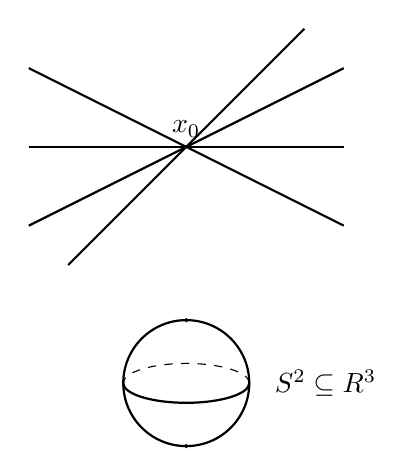
\begin{tikzpicture}
  \coordinate (X0) at (0,1.5);
  \node[above] at (X0) {$x_0$};
  \draw[thick] (-2, 0.5) -- (2, 2.5);
  \draw[thick] (-2, 1.5) -- (2, 1.5);
  \draw[thick] (-2, 2.5) -- (2, 0.5);
  \draw[thick] (-1.5, 0) -- (1.5, 3);
  
  \begin{scope}[yshift=-1.5cm]
    \draw[thick] (0,0) circle (0.8);
    \draw[dashed] (0.8,0) arc (0:180:0.8 and 0.25);
    \draw[thick] (-0.8,0) arc (180:360:0.8 and 0.25);
    \node[right] at (1, 0) {$S^2 \subseteq \mathbb{R}^3$};
    \filldraw (0,0.8) circle (0.5pt); 
    \filldraw (0,-0.8) circle (0.5pt); 
  \end{scope}
\end{tikzpicture}
\caption{Representación gráfica de la intersección en $x_0$ y la esfera $S^2$.}
\end{figure}

\begin{proof}
Vemos claramente que $X$ es arco-conexo (se deduce de manera obvia a partir de las hipótesis).
Sea $x_0 \in \bigcap_{i \in \Lambda} V_i$, se tiene que $\pi_1(X) \cong \pi_1(X, x_0)$.
Sea $\alpha \in C_{x_0}(X)$, $\alpha: I \longrightarrow X$ continua, $\alpha(0)=\alpha(1)=x_0$. Debemos probar que $\alpha \simeq_{\{0,1\}} c_{x_0}$.

Sea $\mathcal{U} = \{\alpha^{-1}(V_i)\}_{i \in \Lambda}$. Vemos que $\mathcal{U}$ es un recubrimiento abierto de $I$. Por el Lema de Lebesgue, $\exists \delta > 0 / \forall x \in I, \exists i(x) \in \Lambda$ tal que $B(x,\delta) \subseteq \alpha^{-1}(V_{i(x)})$. Equivalentemente:
$\exists 0 = t_0 < t_1 < \dots < t_n = 1$ tal que $[t_{j-1}, t_j]$ está contenido en algún elemento de $\mathcal{U}$, $\forall j=1 \dots n$. Es decir:
$\exists 0 = t_0 < t_1 < \dots < t_n = 1$ tal que $\forall j \in \{1 \dots n\}$, existe un $V_j \in \{V_i\}_{i \in \Lambda}$ tal que $\alpha([t_{j-1}, t_j]) \subseteq V_j$.

\begin{figure}[htbp]
\centering
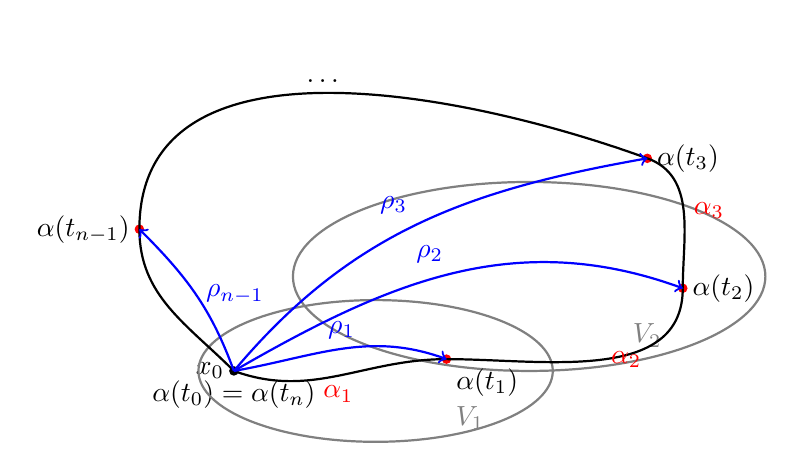
\begin{tikzpicture}[scale=1.5]
  \coordinate (X0) at (0,0);
  \node[below] at (X0) {$\alpha(t_0)=\alpha(t_n)$};
  \node[left] at (X0) {$x_0$};
  \filldraw (X0) circle (1pt);

  \draw[gray, thick] (1.2, 0) ellipse (1.5 and 0.6);
  \node[gray] at (2, -0.4) {$V_1$};
  
  \draw[gray, thick] (2.5, 0.8) ellipse (2 and 0.8);
  \node[gray] at (3.5, 0.3) {$V_2$};

  \coordinate (T1) at (1.8, 0.1);
  \coordinate (T2) at (3.8, 0.7);
  \coordinate (T3) at (3.5, 1.8);
  \coordinate (TN) at (-0.8, 1.2);
  
  \filldraw[red] (T1) circle (1pt) node[black, below right] {$\alpha(t_1)$};
  \filldraw[red] (T2) circle (1pt) node[black, right] {$\alpha(t_2)$};
  \filldraw[red] (T3) circle (1pt) node[black, right] {$\alpha(t_3)$};
  \filldraw[red] (TN) circle (1pt) node[black, left] {$\alpha(t_{n-1})$};

  \draw[thick] (X0) to[out=-20, in=180] node[midway, below, red] {$\alpha_1$} (T1);
  \draw[thick] (T1) to[out=0, in=-90] node[midway, right, red] {$\alpha_2$} (T2);
  \draw[thick] (T2) to[out=90, in=-20] node[midway, right, red] {$\alpha_3$} (T3);
  \draw[thick] (T3) to[out=160, in=90] node[midway, above] {$\dots$} (TN);
  \draw[thick] (TN) to[out=-90, in=135] (X0);
  
  \draw[blue, thick, ->] (X0) to[out=10, in=160] node[midway, above] {$\rho_1$} (T1);
  \draw[blue, thick, ->] (X0) to[out=30, in=160] node[midway, above left] {$\rho_2$} (T2);
  \draw[blue, thick, ->] (X0) to[out=50, in=190] node[midway, above left] {$\rho_3$} (T3);
  \draw[blue, thick, ->] (X0) to[out=110, in=-45] node[midway, right] {$\rho_{n-1}$} (TN);
\end{tikzpicture}
\caption{Descomposición del lazo $\alpha$ en $\alpha_j$ y caminos $\rho_j$.}
\end{figure}

Para cada $j$:
1) $\alpha(t_1) \in V_1 \cap V_2$ arco-conexo, $x_0 \in V_1 \cap V_2 \longrightarrow \exists \rho_1: I \longrightarrow V_1 \cap V_2 / \rho_1(0)=x_0, \rho_1(1)=\alpha(t_1)$.
2) $\alpha(t_2) \in V_2 \cap V_3$ arco-conexo, $x_0 \in V_2 \cap V_3 \longrightarrow \exists \rho_2: I \longrightarrow V_2 \cap V_3 / \rho_2(0)=x_0, \rho_2(1)=\alpha(t_2)$.
$\dots$
n-1) $\alpha(t_{n-1}) \in V_{n-1} \cap V_n$ arco-conexo, $x_0 \in V_{n-1} \cap V_n \longrightarrow \exists \rho_{n-1}: I \longrightarrow V_{n-1} \cap V_n / \rho_{n-1}(0)=x_0, \rho_{n-1}(1)=\alpha(t_{n-1})$.

Sea $j \in \{1 \dots n\}: \alpha|_{[t_{j-1}, t_j]}$. Sea $\alpha_j: I \longrightarrow X$ tal que $s \longmapsto \alpha((1-s)t_{j-1} + st_j)$.

\begin{figure}[htbp]
\centering
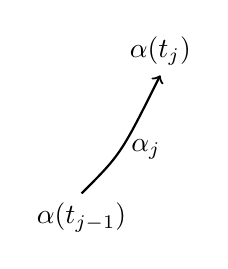
\begin{tikzpicture}
  \coordinate (A) at (0,0);
  \coordinate (B) at (1,1.5);
  \draw[thick, ->] (A) .. controls (0.5, 0.5) .. (B) node[midway, right] {$\alpha_j$};
  \node[below] at (A) {$\alpha(t_{j-1})$};
  \node[above] at (B) {$\alpha(t_j)$};
\end{tikzpicture}
\caption{Detalle del sub-camino $\alpha_j$.}
\end{figure}

Lema: $\exists q: I \longrightarrow I$ continua, $q(0)=0, q(1)=1$ de manera que $\alpha_1 * \dots * \alpha_n = \alpha \circ q$.
Sabemos que $[\alpha] = [\alpha \circ q]$. Por tanto:
$$[\alpha] = [\alpha \circ q] = [\alpha_1 * \alpha_2 * \dots * \alpha_n]$$
$$= [\alpha_1 * \rho_1^{-1} * \rho_1 * \alpha_2 * \rho_2^{-1} * \rho_2 * \alpha_3 * \rho_3^{-1} * \dots * \rho_{n-2} * \alpha_{n-1} * \rho_{n-1}^{-1} * \rho_{n-1} * \alpha_n]$$
$$= [\alpha_1 * \rho_1^{-1}] \cdot [\rho_1 * \alpha_2 * \rho_2^{-1}] \cdot [\rho_2 * \alpha_3 * \rho_3^{-1}] \cdot \dots \cdot [\rho_{n-2} * \alpha_{n-1} * \rho_{n-1}^{-1}] \cdot [\rho_{n-1} * \alpha_n]$$

Donde cada corchete está en $C_{x_0}(V_j)$ respectivamente.
Por hipótesis cada $V_j$ es simplemente conexo, por lo que cada uno se anula a $[c_{x_0}]$. Por tanto $[\alpha] = [c_{x_0}]$.

\begin{figure}[htbp]
\centering
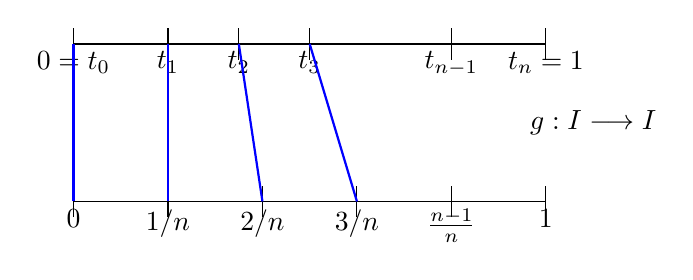
\begin{tikzpicture}[xscale=6, yscale=2]
  \draw (0,1) -- (1,1);
  \draw (0,0.9) -- (0,1.1) node[below=5pt] {$0=t_0$};
  \draw (0.2,0.9) -- (0.2,1.1) node[below=5pt] {$t_1$};
  \draw (0.35,0.9) -- (0.35,1.1) node[below=5pt] {$t_2$};
  \draw (0.5,0.9) -- (0.5,1.1) node[below=5pt] {$t_3$};
  \draw (0.8,0.9) -- (0.8,1.1) node[below=5pt] {$t_{n-1}$};
  \draw (1,0.9) -- (1,1.1) node[below=5pt] {$t_n=1$};

  \draw (0,0) -- (1,0);
  \draw (0,-0.1) -- (0,0.1) node[below=5pt] {$0$};
  \draw (0.2,-0.1) -- (0.2,0.1) node[below=5pt] {$1/n$};
  \draw (0.4,-0.1) -- (0.4,0.1) node[below=5pt] {$2/n$};
  \draw (0.6,-0.1) -- (0.6,0.1) node[below=5pt] {$3/n$};
  \draw (0.8,-0.1) -- (0.8,0.1) node[below=5pt] {$\frac{n-1}{n}$};
  \draw (1,-0.1) -- (1,0.1) node[below=5pt] {$1$};

  \draw[blue, thick] (0,0) -- (0,1);
  \draw[blue, thick] (0.2,0) -- (0.2,1);
  \draw[blue, thick] (0.4,0) -- (0.35,1);
  \draw[blue, thick] (0.6,0) -- (0.5,1);
  
  \node at (1.1, 0.5) {$g: I \longrightarrow I$};
\end{tikzpicture}
\caption{Mapeo de subintervalos para la función de reparametrización $g$.}
\end{figure}
\end{proof}

\begin{proposicion}{}{corolario_sn}
Para $n \ge 2$, $S^n$ es simplemente conexo.
\end{proposicion}

\begin{proof}
Recordemos que $S^n \subseteq \mathbb{R}^{n+1}$, $S^n := \{ (x_1, \dots, x_{n+1}) \in \mathbb{R}^{n+1} / x_1^2 + \dots + x_{n+1}^2 = 1 \}$.
Supongamos $n \ge 2$:
Tomamos $V_1 := S^n \setminus \{(0, \dots, 0, 1)\} = S^n \setminus \{N\}$ y $V_2 := S^n \setminus \{(0, \dots, 0, -1)\} = S^n \setminus \{S\}$.
\begin{itemize}
\item $V_1 \cap V_2 = S^n \setminus \{N, S\} \cong S^{n-1} \times \mathopen]-1, 1\mathclose[$. $S^{n-1} \times \mathopen]-1, 1\mathclose[$ son arco-conexos, luego también lo es.
\item $V_1, V_2$ contráctiles $\longrightarrow$ luego son simplemente conexos.
\end{itemize}
Por aplicación directa del teorema anterior concluimos que $S^n$ es simplemente conexo.

\begin{figure}[htbp]
\centering
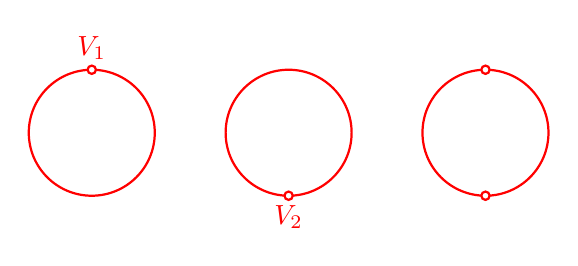
\begin{tikzpicture}
  \draw[red, thick] (0,0) circle (0.8);
  \filldraw[white] (0,0.8) circle (1.5pt);
  \draw[red, thick] (0,0.8) circle (1.5pt);
  \node[above, red] at (0,0.8) {$V_1$};

  \draw[red, thick] (2.5,0) circle (0.8);
  \filldraw[white] (2.5,-0.8) circle (1.5pt);
  \draw[red, thick] (2.5,-0.8) circle (1.5pt);
  \node[below, red] at (2.5,-0.8) {$V_2$};

  \draw[red, thick] (5,0) circle (0.8);
  \filldraw[white] (5,0.8) circle (1.5pt);
  \draw[red, thick] (5,0.8) circle (1.5pt);
  \filldraw[white] (5,-0.8) circle (1.5pt);
  \draw[red, thick] (5,-0.8) circle (1.5pt);
\end{tikzpicture}
\caption{Visualización de $V_1$, $V_2$ y su intersección para el caso de $S^1$.}
\end{figure}

La prueba del corolario no funciona cuando $n=1$, ya que $V_1 \cap V_2$ no es arco-conexo. Veremos que $\pi_1(S^1) \cong (\mathbb{Z}, +)$.
\end{proof}